\documentclass[a4paper]{article}
%% Language and font encodings
\usepackage[english]{babel}
\usepackage[utf8x]{inputenc}
\usepackage[T1]{fontenc}

%% Sets page size and margins
\usepackage[a4paper,top=3cm,bottom=2cm,left=3cm,right=3cm,marginparwidth=1.75cm]{geometry}

%% Useful packages
\usepackage{amsmath}
\usepackage{graphicx}
\usepackage[colorinlistoftodos]{todonotes}
\usepackage[colorlinks=true, allcolors=blue]{hyperref}



\title{Actividad 9}
\author{Isaac Neri Gómez Sarmiento}
\date{01 de Mayo de 2018}

\begin{document}
\maketitle


\section{Introducción}
En esta Actividad aprenderemos a usar Maxima, el cual es un software de álgebra computacional.
Este tipo de software permite al usuario manipular expresiones simbólicas y numéricas y graficar.
Además, permite integrar, derivar, resolver ecuaciones diferenciales, realizar operaciones matriciales,
etc.
El software tuvo su origen en un proyecto del MIT llamado proyecto MAC (Proyect on Mathematics
and Computation).

\section{Sintáxis básico}

La primera línea de comando en Maxima está enumerado de la siguiente forma cuando es una entrada: \textbf{\%i1 } y cuando
es salida: \textbf{\%o1 }.
Para utilizar algún resultado, se puede guardar en una variable o también con el caracter \textbf{\%},
el cual guarda el valor más reciente calculado.
Si queremos que el resultado no se imprima en pantalla, en lugar de escribir \textbf{;} al final de una línea, escribimos \textbf{\$}.

Los dos tipos de números que acepta máxima son reales y complejos. En los reales se incluyen
los enteros, racionales e irracionales. Los números irracionales como sqrt(2) o log(2) se expresan
de esa forma y no en números decimales, para expresarlo en formato decimal se utiliza el siguiente
comando:

\begin{verbatim}
(%i1) float(sqrt(2))
(%o1) 1.414213562373095
\end{verbatim}


Por otra parte, se pueden racionalizar numeros decimales, es decir expresar en forma de fraccion
con el comando \textbf{rationalize()}. Por ejemplo, si queremos racionalizar el número .375, entonces
escribimos en la linea de comandos \textbf{rationalize(.375)} y tendremos la salida como: $\frac{3}{8}$.
Para poder asignar a una variable un valor u otros objetos, se utiliza el símbolo : y no el igual.
Una consideración que se debe de hacer es que Maxima es sensible a las mayúsculas.

Para remover un valor asignado a alguna variable se utiliza el comando \textbf{remvalue(a)} y para
remover los valores asignados de todas las variable creadas se utiliza el comando \textbf{remvalue(all)}. 
Para dar un valor a una variable de una expresión, se utiliza el comando \textbf{subst()}. Por ejemplo:


\begin{verbatim}
(%i12) a:x**3+x**2+x+1;
(a) x^3+x^2+x+1
(%i13) subst(x=2,a);
(%o13) 15
\end{verbatim}

A una variable se le puede asociar una ecuación, por ejemplo:

\begin{verbatim}
(%i16) SegundaleyNewton: F=m*a;
(SegundaleyNewton) F=a*m
(%i21) subst([m=10, ’a=9.8], SegundaleyNewton);
(%o21) F=98.00000000000001
\end{verbatim}

La razón por la cual se le puso un apostrofe a la izquierda de "a " es para evitar que se
remplazara para asignarle la expresión antes creada a: x**3+x**2+x+1.
Para realizar una lista, simplemente se encierra en corchetes y se separan por coma los elementos contenidos en ella, por ejemplo:

\begin{verbatim}
numeros: [1,2,3,4,5,6,7,8,9,10]$
(%i26) cuadrados: numeros**2;
(cuadrados) [1,4,9,16,25,36,49,64,81,100]
\end{verbatim}

Para seleccionar un elemento de la lista se utiliza el nombre de la variable y en corchetes
e indice del valor. Para obtener una lista de  varios números al cuadrado, podemos utilizar una iteración:

\begin{verbatim}
(%i29)	makelist(i**2, i, 1, 10);
(%o29) [1,4,9,16,25,36,49,64,81,100]
\end{verbatim}

Maxima identifica constantes tales como el numero $\pi$ usando \%pi, el número de Euler $e$ usando \%e y el número imaginario $i=\sqrt[2]{-1}$ usando \%i. 

La función \textbf{allroots()} proporciona todas las raíces de un polinomio al igual que la función \textbf{solve()} por ejemplo:

\begin{verbatim}
(%i26)	allroots(x**2-2*x-1);
(%o26)	[x=-0.4142135623730951,x=2.414213562373095]

(%i24)	solve(x**2-2*x-1);
(%o24)	[x=1-sqrt(2),x=sqrt(2)+1]
\end{verbatim}
La diferencia es que la primera da una solución aproximada, mientras que la segunda una solución exacta.

Para resolver un sistema de ecuaciones, sea lineal o no lineal, se tienen que definir las ecuaciones involucradas y utilizar la función \textbf{solve()}. Por ejemplo, para resolver el sistema con las ecuaciones de un ejercicio de determinación de corriente eléctrica en un circuito se hace lo siguiente:

\begin{verbatim}
(%i27)	eqA: -3*I1+9*I2+2*I6=-4$
(%i28)	eqB: 3*I1+2*I2+9*I6=-2$
(%i32)	eqC: -6*I1-4*I2+4*I6=-22$
(%i33)	solve([eqA, eqB, eqC], [I1, I2, I6]);
(%o33)	[[I1=27/11,I2=7/11,I6=-13/11]]
\end{verbatim}

Para graficar en el plano cartesiano, se proporciona el siguiente ejemplo:

\begin{verbatim}
wxplot2d([sin(x),-cos(x)], [x,-5,5], [y,-1.5,1.5])$
\end{verbatim}


\begin{figure}[ht!]
\centering
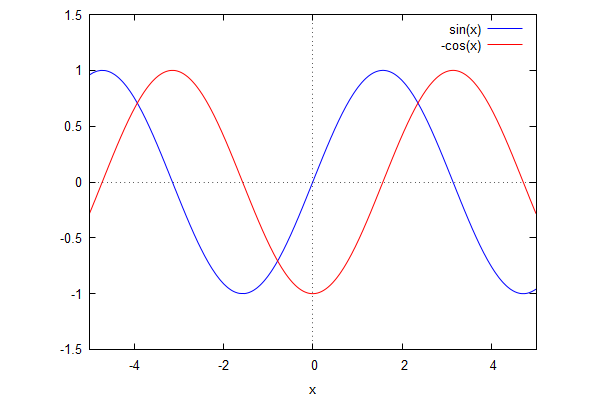
\includegraphics[width=0.5\textwidth]{grafica2d.png}
\end{figure}


Para graficar en R3, se proporciona otro ejemplo:

\begin{verbatim}
wxplot3d(sin(sqrt(x^2 + y^2))/sqrt(x^2 + y^2), [x,-12,12], [y,-12,12])$
\end{verbatim}

\begin{figure}[ht!]
\centering
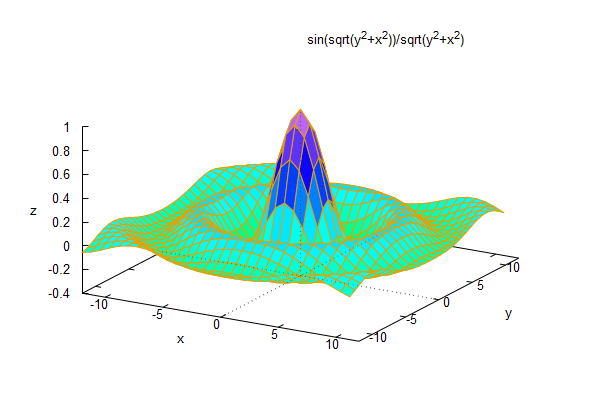
\includegraphics[width=0.5\textwidth]{grafica3d.png}
\end{figure}

\section{Tutorial: Diferenciación}

El comando general para derivar en máxima es:

\begin{verbatim}
diff(expresión, variable, orden de la derivada)
\end{verbatim}

La ventaja del comando es que puedes poner el número de veces que quieres derivar. Por ejemplo si queremos derivar tan(x) 5 veces:

\begin{verbatim}
(%i13)	diff(tan(x), x, 5)
(%o13)	16*sec(x)^2*tan(x)^4+88*sec(x)^4*tan(x)^2+16*sec(x)^6
\end{verbatim}

Para definir una función que queramos derivar lo haremos de la siguiente forma:

\begin{verbatim}
(%i28)	h(x):=csc(x)$
(%i29)	diff(h(x), x, 5);
(%o29)	-61*cot(x)*csc(x)^5-58*cot(x)^3*csc(x)^3-cot(x)^5*csc(x)
\end{verbatim}


Para poder almacenar la derivada de una función f(x) como otra función g(x) se procede de la siguiente forma.

\begin{verbatim}
(%i30)	f(x):=sqrt(tan(cos(x)));
(%i32)	g(x):=subst(t=x, diff(f(t), t));
\end{verbatim}

Para evaluar la derivada , simplemente se sustituye g(x) por g(a), siendo a una constante. 

Existe otra manera para simplificar el proceso de sustitución de variable y derivación, utilizando el siguiente comando:

\begin{verbatim}
NDIFF(f,n):=subst(t=x, diff(f(t), t, n));
\end{verbatim}

Esto lo utilizaremos para graficar la función $sin(x)$ y sus 2 primeras derivadas.

\begin{verbatim}
(%i22)	f(x):=sin(x);
(%i23)	g(x):=NDIFF(f(x),1);
(%i24)	h(x):=NDIFF(f(x), 2);
wxplot2d([f(x), g(x), h(x)], [x, -8,8], [legend, "Función", "1° derivada", "2°da derivada"]
, [title, "Dos primeras derivadas de f(x)=sin(x)"]);
\end{verbatim}

La gráfica resultante es:

\begin{figure}[ht!]
\centering
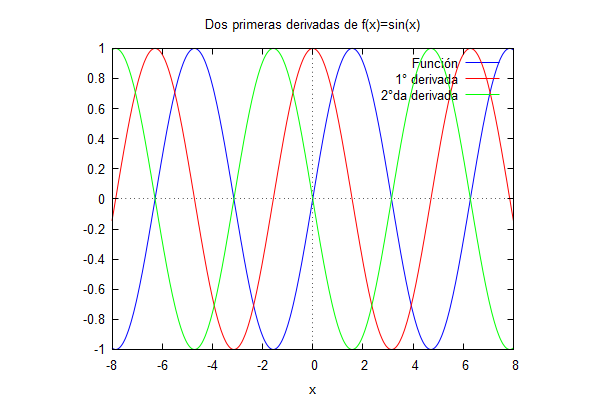
\includegraphics[width=0.5\textwidth]{grafica2derivadas.png}
\end{figure}

\newpage

Para obtener un valor en punto decimal de una derivada evaluada y no solo expresada, se utiliza la función \textbf{float()}. Por ejemplo:

\begin{verbatim}
(%i27)	l(x):=tan(x);

(%i31)	m(x):=subst(t=x, diff(l(t), t));

(%i33)	m(1/sqrt(2));

(%o33)	sec(1/sqrt(2))^2

(%i34)	float(m(1/sqrt(2)));

(%o34)	1.730188078413236
\end{verbatim}






\section{Apéndice}

\textbf{1° ¿Cuál fue tu primera impresión de wxmaxima?}\\

Que tiene algunas funciones similares a las de Wolfram Alpha.

\textbf{2° ¿Crees que esta herramienta puede ser útil en otros de tus cursos?}\\
De hecho sí, mas que nada para facilitar "la talacha" de resolver problemas algebraicos como un sistemas de ecuaciones.

\textbf{3° ¿Qué se te dificultó más en esta actividad?}\\
No hubo nada que se me dificultara de la actividad. Diría yo que donde tarde más fue en escoger un tutorial. 

\textbf{4° ¿Se te hizo compleja esta actividad? ¿Cómo la mejorarías?}\\
No se me hizo compleja. Considero que estuvo bien esta actividad para introducirnos a la sintaxis de Maxima ya que posiblemente la próxima actividad consista en resolver un problema usando Maxima. 


\end{document}